%%%%%%%%%%%%%%%%%%%%%%%%%%%%%%%%%%%%%%%%%%%%%%%%%%%%%%%%%%%%%%%%%%%%%%%%%%%%%%%%
%2345678901234567890123456789012345678901234567890123456789012345678901234567890
%        1         2         3         4         5         6         7         8

\documentclass[conference]{IEEEtran} % [letterpaper, 10 pt, conference]{ieeeconf}  % Comment this line out if you need a4paper

%\documentclass[a4paper, 10pt, conference]{ieeeconf}      % Use this line for a4 paper

\IEEEoverridecommandlockouts                              % This command is only needed if 
                                                          % you want to use the \thanks command

\overrideIEEEmargins                                      % Needed to meet printer requirements.

%In case you encounter the following error:
%Error 1010 The PDF file may be corrupt (unable to open PDF file) OR
%Error 1000 An error occurred while parsing a contents stream. Unable to analyze the PDF file.
%This is a known problem with pdfLaTeX conversion filter. The file cannot be opened with acrobat reader
%Please use one of the alternatives below to circumvent this error by uncommenting one or the other
%\pdfobjcompresslevel=0
%\pdfminorversion=4

% See the \addtolength command later in the file to balance the column lengths
% on the last page of the document

% ==================================================================================
\usepackage{graphics} % for pdf, bitmapped graphics files
\usepackage{epsfig} % for postscript graphics files
%\usepackage{mathptmx} % assumes new font selection scheme installed
%\usepackage{times} % assumes new font selection scheme installed
\usepackage{amsmath} % assumes amsmath package installed
\usepackage{amssymb}  % assumes amsmath package installed
\usepackage{amsfonts} % assumes amsfonts package installed
\usepackage{epstopdf}
\usepackage{color}
\usepackage{comment}
\usepackage{algorithm}
\usepackage{algorithmic}
%\usepackage{algpseudocode}
\renewcommand{\algorithmicrequire}{\textbf{Input:}}  % Use Input in the format of Algorithm  
\renewcommand{\algorithmicensure}{\textbf{Output:}} % Use Output in the format of Algorithm  
%===================================================================================

\newtheorem{example}{Example}
\newtheorem{remark}{Remark}
\newtheorem{definition}{Definition}
\newtheorem{theorem}{Theorem}
\newtheorem{lemma}{Lemma}
\newtheorem{proposition}{\bf Proposition}


%============================================================================
\def \BN {{\em BN}}
\def \BNs {{\em BNs}}
\def \BCN {{\em BCN}}
\def \BCNs {{\em BCNs}}
\newcommand{\rev}[1]{{\color{red}{#1}}}


%=======================================================================
\newcommand{\tl}[1]{\textcolor{blue} {TL: #1 :TL} }

%========================================================================

\title{\LARGE \bf
Online Observability of Boolean Control Networks*
}

\begin{comment}


\author{Guisen Wu$^{1}$ and Liyun Dai$^{1}$ and Taolue Chen$^{2}$% <-this % stops a space
\thanks{*This work was not supported by any organization}% <-this % stops a space
\thanks{$^{1}$Albert Author is with Faculty of Electrical Engineering, Mathematics and Computer Science,
        University of Twente, 7500 AE Enschede, The Netherlands
        {\tt\small albert.author@papercept.net}}%
\thanks{$^{2}$Bernard D. Researcheris with the Department of Electrical Engineering, Wright State University,
        Dayton, OH 45435, USA
        {\tt\small b.d.researcher@ieee.org}}%
}
\end{comment}

\author{\IEEEauthorblockN{Guisen Wu\quad  Liyun Dai*\thanks{*Corresponding author} \quad Zhiming Liu}
\IEEEauthorblockA{\textit{RISE \& School of Computer and Information Science,}\\ \textit{Southwest University}\\
Chongqing, China \\
$\{$wgs233,dailiyun,zhimingliu88$\}$@swu.edu.cn}
\and
\IEEEauthorblockN{Taolue Chen}
\IEEEauthorblockA{\textit{Department of Computer Science and Information Systems} \\
	\textit{Birkbeck, University of London}\\
taolue@dcs.bbk.ac.uk}
\and
\IEEEauthorblockN{Jun Pang}
\IEEEauthorblockA{\textit{Faculty of Science, Technology and Communication} \\
	\textit{University of Luxembourg}\\
jun.pang@uni.lu}
\and
\IEEEauthorblockN{Hongyang Qu}
\IEEEauthorblockA{\textit{Department of Automatic Control and Systems Engineering} \\
	\textit{University of Sheffield}\\
h.qu@sheffield.ac.uk}
}



\begin{document}



\maketitle
\thispagestyle{empty}
\pagestyle{empty}


%%%%%%%%%%%%%%%%%%%%%%%%%%%%%%%%%%%%%%%%%%%%%%%%%%%%%%%%%%%%%%%%%%%%%%%%%%%%%%%%
\begin{abstract}

Four types of observability of Boolean control networks ({\em BCNs}) have been proposed to solve different problems. However, all of them are offline observabilities that we can't adjust the input sequence by observing the output sequence in the process of determining the initial state of BCNs. In this paper, we firstly propose the online observability that it can determine the initial state of BCNs dynamically without presupposing its initial state. The online observability accomplishes this task by deciding input sequence and observing out sequence in every time step. The node values of {\em BCNs} update at discrete time, then we use the time step to represent the discrete time. Compare with offline observabilities, the online obsevability can determine the initial state of some biological systems which can be checked at most once. %We define the concepts of deduce function, $K$ steps deterministic and the formal definition of online observability of BCNs. We also define the supertree and directed graph to determine online observability for BCNs. 
\end{abstract}


\begin{keywords}

Boolean control networks, online observability, directed graph, supertree%, find shortest path, avoid entering critical states. 

\end{keywords}

%\section{ssssss}
\label{sec;one}
ssssssss

ss

s

s
s

d
d
f


%%%%%%%%%%%%%%%%%%%%%%%%%%%%%%%%%%%%%%%%%%%%%%%%%%%%%%%%%%%%%%%%%%%%%%%%%%%%%%%%
\section{INTRODUCTION}

In 1960s, Nobel Prize winners Jacob and Monod found that  ``Any cell contains a number of `regulatory' genes that act as switches and can turn one another on and off. If genes can turn one another on and off, then you can have genetic circuits.'' \cite{Waldrop1992Complexity,cheng2009controllability}. Inspired by these Boolean-type actions in genetic circuits, the Boolean networks ({\em BNs}) is firstly proposed by Kauffman \cite{Kauffman1968Metabolic} for modeling nonlinear and complex biological systems. Some general descriptions of the \BNs\ and its applications to biological systems can be found in Kauffman. Since then research interests in  \BNs\ have been motivated by the large number of natural and artificial systems. These natural and artificial systems describing variables display only two distinct configurations, and hence these describing variables take only two values, i.e., $\{0,1\}$  \cite{Akutsu2000Inferring, Shmulevich2002From, Faur2006Dynamical,Green2007The,Lou2010Multi,Fornasini2013Observability}.

When extenal regulation or perturbation is considered, \BNs\ are naturally extended to Boolean control networks ({\em BCNs}) \cite{Ideker2001A}. The study on control-theoretic problems of \BCNs\ can date back to 2007 \cite{Akutsu2007Control}. The work above also proves that the problem of determining the controllability of \BCNs\ is {\em NP}-hard in the number of nodes. Furthermore, it points out that ``One of the major goals of systems biology is to develop a control theory for complex biological systems.'' Since then, the study on control-theoretic problems in the areas of \BNs\ and \BCNs\ has drawn great attention \cite{cheng2009controllability, Zhao2010Input, Cheng2011Identification, Cheng2011Analysis,Fornasini2013Observability}. Furthermore, controllability and observability are basic control-theoretic problems. In 2009, an algebraic framework to deal with both \BNs\ and \BCNs\ by using \emph{semi-tensor product} (STP) of matrices has been developed in \cite{cheng2009controllability}. Moreover they give equivalent conditions for controllability of \BCNs\ and observability of controllable {\em BCNs}. To date, there are four types of observability have been proposed. 

\begin{enumerate}
	\item The first type of observability proposed in 2009 \cite{cheng2009controllability} means that every initial state can be determined by an input sequence.
	
	\item 
	The second observability proposed in 2010 \cite{Zhao2010Input} stands for that for every two distinct initial states, there exists an input sequence which can distinguish them, and this observability is determined in \cite{Li2015Controllability}.
	
	\item The third observability proposed in 2011 \cite{Cheng2011Identification} states that there is an input sequence that determines the initial state.
	
	\item  The fourth observability proposed in 2013 \cite{Fornasini2013Observability} is essentially the observability of linear control systems, i.e., every sufficient long input sequence can determine the initial state.
\end{enumerate}
 

%\tl{can you state the four types observability clearly and formally here?}

%\rev{****input sequence***}
In abovementioned definitions an input is not the value of an input-node, but it represents the values of all input-nodes of the \BCN\ on a time step. Therefore an input is a vector of the values of all input-nodes of the \BCN\ on a time step. An input sequence consists of several inputs in sequential time steps. We will give the formal definition of four observabilities in the following pages. All of four existing types of observability of \BCNs\ are offline observabilities which means that they can't adjust the input sequence by observing the output sequence in the process of determining the initial state of {\em BCNs}. Therefore, we propose the online observability that we can determine the initial state of \BCNs\ dynamically. The online observability decides the input sequence and observes the out sequence step by step.
\subsubsection*{Contribution}
Firstly, we give the formal definition of online observability of {\em BCNs}. Secondly, we provide two algorithms to determine the online observability for {\em BCNs}. Finally, we introduce some applications of the online observability of {\em BCNs} and advantages of online observability compared with offline observabilities. %\rev{***Compare with offline observabilities****} 
\subsubsection*{Structure}
The remainder of this paper is organized as follows. {\em Section II} introduces necessary preliminaries about {\em BCNs}, algebraic forms of \BCNs\ and the four existing kinds of observability of {\em BCNs}. {\em Section III} presents the definition of deduce function, $K$ steps deterministic and online observability of {\em BCNs}. {\em Section IV} presents how to determine the online observability of \BCNs\ by super tree and directed graph. {\em Section V} talks about some applications of the online observability of {\em BCNs}. We also compare the online observability with offline observabilities in this section. {\em Section VI} ends up  with the introduction of some future works.

%\tl{I will try to rewrite the intro.}

%==============================================================================================================
\section{PRELIMINARIES}
In this section we introduce the definition of \BCNs\ and their algebraic form, and the existed four kinds of observability of {\em BCNs}.



\subsection{Boolean Control Networks}

A Boolean control network can be described as a directed graph together with logical equations to describe the updating rules of the nodes in the graph, the definition of {\em BCN} is as follows. 

\begin{definition}
(\cite{Ideker2001A}) A \BCN\ consists of input-nodes, state-nodes, output-nodes, and directed edges which connect nodes. A node in \BCN\ can take a logic value from $\{0,1\}$ at a discrete time 0, 1, 2,\ldots. For one directed edge from node $v_i$ to node $v_j$ means that the logic value of $v_j$ at time step $t+1$ is affected by the value of $v_i$ at time step $t$ or $t+1$. 
\end{definition}


Note that one can only know whether or not a node is affected by another node from the network graph. Different \BCNs\ may have the same structure, in order to determine a \BCN\ uniquely, logical equations are also needed to describe the specific updating rules of {\em BCNs}.

 
 \begin{figure}[thpb]
      \centering
      \framebox{\parbox{3in}{
		\centerline{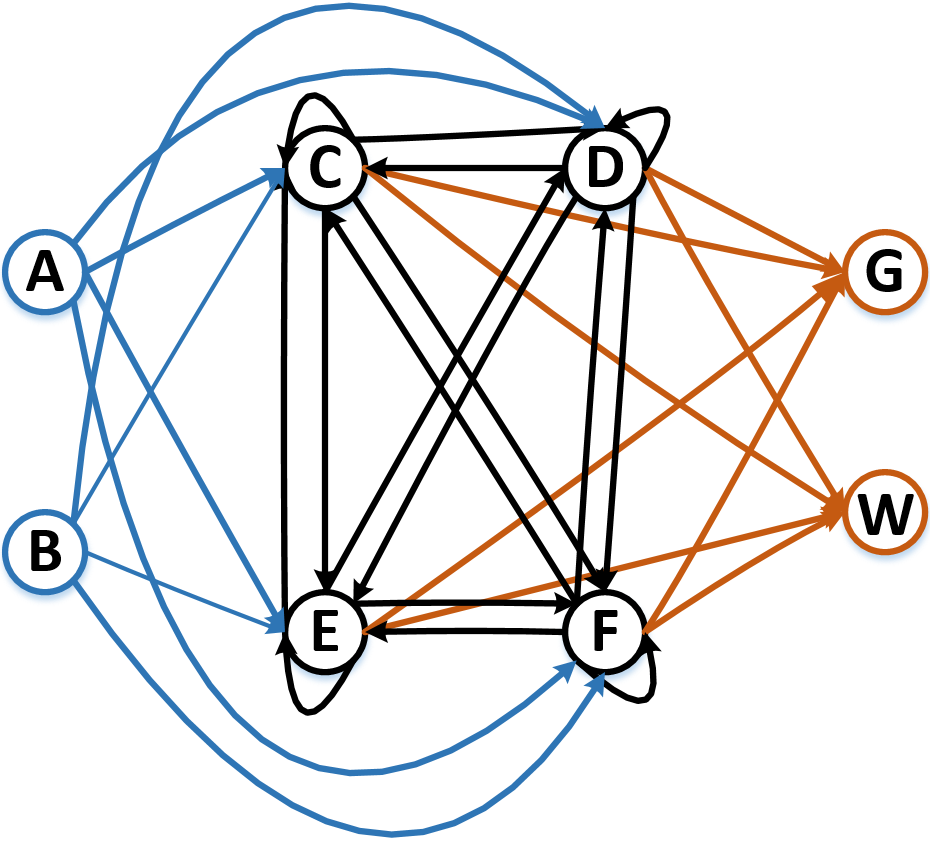
\includegraphics[scale=0.23]{figures/Fig1.png}}
	}}
      
      \caption{A Boolean control network with two input-nodes $A$ and $B$, four state-nodes $C$, $D$, $E$ and $F$, and two output-nodes $G$, $W$. We use blue, black and orange, to distinguish three kinds of nodes and three kinds of edges.}
      \label{fig:1}
  \end{figure}

Firstly, we give a simple example to describe {\em BCN}.

\begin{example}
	In {\em  Fig.\ref{fig:1}} we have a \BCN\ with two input-nodes $A$ and $B$, four state-nodes $C$, $D$, $E$ and $F$, and two output-nodes $G$, $W$. The updating rules of the \BCN\ shown in the edges of {\em Fig.\ref{fig:1}}, and they are also described as truth table ({\em Fig.\ref{fig:2}}). The reason why we use truth table to describe the updating rules of the \BCN\ is that,  this form will be more convenient for \BCN\ to convert into its aglebraic form.
	
	For convenience, we will use this example in the whole paper to explain various concepts we introduce.
  \begin{figure}[thpb]
      \centering
      \framebox{\parbox{3in}{
		\centerline{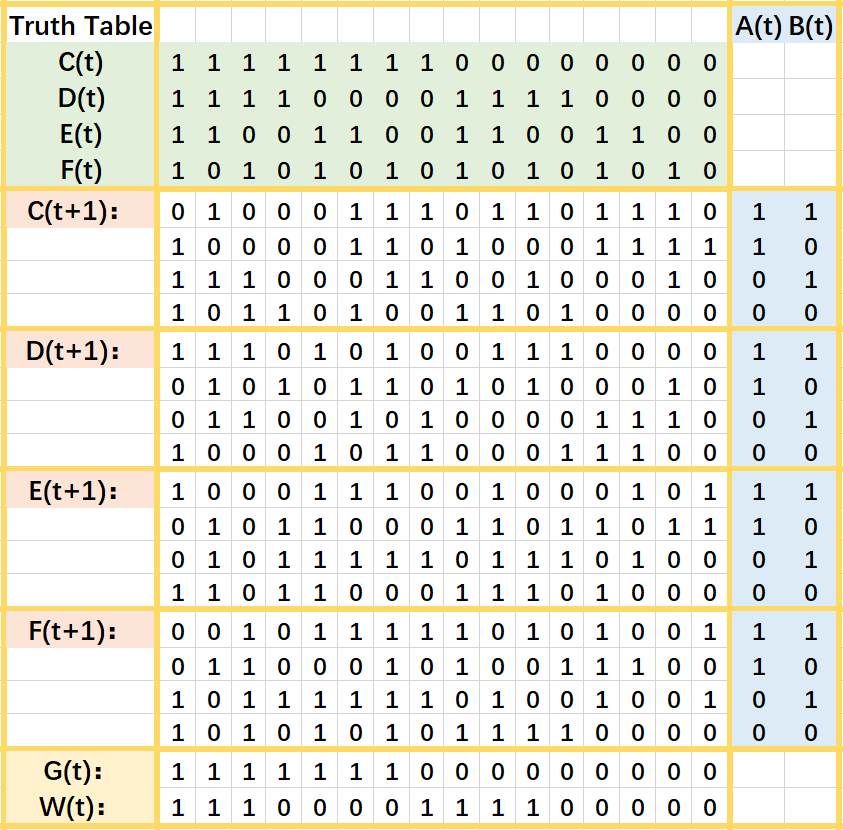
\includegraphics[scale=0.26]{figures/Fig21.png}}
	}}
      
      \caption{The truth table which describe the updating rules of the \BCN\ shown in {\em Fig.\ref{fig:1}}.}
      \label{fig:2}
   \end{figure}
\end{example}   


%==============================================================================================================
\subsection{The Algebraic Forms of BCNs}
To better illustrate the concept of algebraic forms, in this paper, we investigate the following \BCN\ assumes to has $n$ state-nodes, $m$ input-nodes and $q$ output-nodes. Then the updating rules of the \BCN\ can be described as following formulas:
\begin{equation}
\begin{split}
s(t+1)=&f(i(t),s(t))\\
o(t)=&h(s(t))
\end{split}
\label{equ:1}
\end{equation}
$s(t)\in \mathbb{B}^n$ are state-nodes; $i(t)\in \mathbb{B}^m$ are input-nodes; $o(t)\in \mathbb{B}^q$ are output-nodes; $f:\mathbb{B}^{n+m}\mapsto \mathbb{B}^n$ and $h:\mathbb{B}^n\mapsto \mathbb{B}^q$ are logical functions that represent the updating rules of {\em BCNs}. Where $\mathbb{B}$ : the set $\{0,1\}$; $t=0,1,...$ represents the discrete time. 

Therefore in the previously mentioned example, we have $C(t), D(t), E(t), F(t)\in s(t)$; $A(t), B(t)\in i(t)$ and $G(t), W(t)\in o(t)$; $n=4$, $m=2$ and $q=2$; $f$ and $h$ are described in the truth table ({\em Fig.\ref{fig:2}}). 

The {\em STP} of matrices can be used to represent the algebraic forms of {\em BCNs} \cite{cheng2009controllability}, the definition of {\em STP} is as follows.

\begin{definition}[STP] 
	\cite{Cheng2011Analysis} Let $X\in\mathbb{R}_{m\times n}$, $Y\in\mathbb{R}_{p\times q}$ and $\alpha=lcm(n,p)$ be the least common multiple of $n$ and $p$. The STP of $X$ and $Y$ is defined as $X\ltimes Y=(X\otimes I_{\alpha/n})(Y\otimes I_{\alpha/p})$, where $\otimes$ denotes the Kronecker product. 
\end{definition}

After introduce the definition of {\em STP} of matrices,  we introduce some related notations at first \cite{Zhang2016Observability}:
\begin{itemize}
  \item $\delta^i_n$: the $i$-th column of the identity matrix $I_n$;
  \item $\Delta_n$: the set $\{\delta^1_n,...,\delta^n_n \}$; 
  \item $\delta_n \left[i_1,...,i_s\right]$: $\left[\delta^{i_1}_n,...,\delta^{i_s}_n\right]\left(i_1,...,i_s\in\left\{1,2,...,n\right\}\right)$ the logical matrix;
  \item  $L_{n\times s}$: the set of $n\times s$ logical matrices.
\end{itemize}


Using {\em STP} of matrices, {\bf (\ref{equ:1})} can be quivalently represented in the following algebraic form:
\begin{equation}
\begin{split}
s(t+1)=&L\ltimes{i(t)}\ltimes{s(t)}\\
o(t)=&H\ltimes{s(t)}
\end{split}
\label{equ:2}
\end{equation}
where $s(t)\in\Delta_N$, $i(t)\in\Delta_M$, and  $o(t)\in\Delta_Q$ denote the states, inputs and outputs respectively the same as in {\em (\ref{equ:1})}, but they are with vector forms; $L\in L_{N\times\left(NM\right)}$; $H\in L_{Q\times N}$ denote the relation matrices; that $N=2^n$, $M=2^m$, and $Q=2^q$. Since {\em STP} keeps most properties of the conventional product \cite{Cheng2011Analysis}, the associative law, the distributive law, etc., we usually omit the symbol ``$\ltimes$'' hereinafter.

To construct {\em (\ref{equ:2})} we give each logical value a vector form as: $T = 1 \scriptsize{\sim} \delta_2^1$, $F = 0 \scriptsize{\sim} \delta_2^2$, therefore the logical variable $A(t)$ takes value from thiese two vectors, i.e., $A(t)\in D=\{\delta_2^1, \delta_2^2\}$. Using the {\em STP} of matrices, $i(t)=i_1(t)...i_m(t)$; $s(t)=s_1(t)...s_n(t)$; $o(t)=o_1(t)...o_q(t)$. And according to \cite{Cheng2003Semi}, for each logical function of state-nodes $f_p(i_1(t),...,i_m(t),s_1(t),...,s_n(t))$ there exists a structure matrix $L_p\in L_{2\times {NM}}$, that
\begin{equation}
\begin{split}
f_p(i_1(t),...,i_m(t),s_1(t),...,s_n(t))=L_pi(t)s(t)
\end{split}
\end{equation}
for $n$ state-nodes, we have $n$ logical matrices for all of the state-nodes $L_1,...,L_n$. If for each state-node ($s_p(t)$) the logical matrix $L_p=[\delta_2^{p_1},...,\delta_2^{p_{NM}}]$, and for all state-nodes ($s(t)$) the logical matrix $L=[\delta_N^{R_1},...,\delta_N^{R_{NM}}]$, then we have $\delta_N^{R_1}=\delta_2^{1_1}...\delta_2^{n_1}$;...; $\delta_N^{R_{NM}}=\delta_2^{1_{NM}}...\delta_2^{n_{NM}}$. We can construct the logical matrix $H$ in the similar way.

Then the \BCN\ whose structure is depicted in {\em Fig.\ref{fig:1}}, and whose updating rules is described as truth table in {\em Fig.\ref{fig:2}}, can be represented with the algebraic form:
\begin{equation}
\begin{split}
s(t+1) =&\delta_{16}[\alpha]i(t)s(t)\\
o(t) =&\delta_4[\beta]s(t)\\
\end{split}
\end{equation}
where $\alpha=\{10,4,11,16,9,5,1, 7,15,2,3,12,7,6,8,13,8,9,\\15,10,14,4,3,16,1,14,12,13,5,7,2,6,7,2,3,13,13,9,5,1,\\16,13 ,6,14,11,10,4,15,1,14 ,7,6,9 ,8,11,12,5,5,13,3,10,\\12,16,16\}$ and $\beta=\{1,1,1,2,2,2,2,3,3,3,3,4,4,4,4,4\}$; $t\in \mathbb{N}$; $s\in \Delta_{16}$; $i\in \Delta_4$; $o\in \Delta_4$.
\subsection{Four Existing Observability of BCNs}
In this section we introduce four existing kinds of observability of {\em BCNs}. Let $\Delta_N$, $\Delta_M$, $\Delta_Q$ be three alphabets, for all $s_0\in \Delta_N$ and all $p\in \mathbb{Z}_+$; $\infty$ is the infinite natural numbers. In order to introduce four existing kinds of observability of {\em BCNs}, we define the mappings \cite{Zhang2016Observability}:
\begin{equation}
\begin{split}
L^p_{s_0} &: (\Delta_M)^p\mapsto(\Delta_N)^p, u_0 . . . u_{p-1} \mapsto s_1 . . .\, s_p\\
L^{\infty}_{s_0} &: (\Delta_M)^{\infty}\mapsto(\Delta_N)^{\infty}, u_0 u_1 . . .  \mapsto s_1 s_2 . . .
\end{split}
\end{equation}
\begin{equation}
\begin{split}
(HL)^p_{s_0} &: (\Delta_M)^p\mapsto(\Delta_Q)^p, u_0 . . . u_{p-1} \mapsto o_1 . . .\, o_p\\
(HL)^{\infty}_{s_0} &: (\Delta_M)^{\infty}\mapsto(\Delta_Q)^{\infty}, u_0 u_1 . . .  \mapsto o_1 o_2 . . .
\end{split}
\end{equation}

For all  $p\in \mathbb{Z}_+$, all $U=u_1 ... u_p \in(\Delta_M)^p$, and all $1\ge i \ge j \ge |U|$, we use U[i,j] to denote the word $u_i ... u_j$ as the input sequence. Then four existing kinds of observability of BCNs can be define as: 
\begin{definition}
The first kind of observability is that, \BCN\ is called observable, if for every initial state $s_0 \in \Delta_N$, there exists an input sequence $U\in(\Delta_M)^p$ for some $p\in \mathbb{Z}_+$ such that for all states $s_0\neq {s'}_0\in \Delta_N$, $Hs_0=H{s'}_0$ implies $(HL)^p_{s_0}(U)\neq (HL)^p_{{s'}_0}(U)$ \cite{cheng2009controllability}.
\end{definition}

So the first observability means that if a \BCN\ is observable then every initial state of the \BCN\ can be determined by an input sequence. But we can only use the corresponding input sequence of a state to check whether this state is the initial state of the {\em BCN} or not.
\begin{definition}
	The second kind of observability is that a \BCN\ is called observable if for any distinct states $s_0$, ${s'}_0 \in \Delta_N$, there exists an input sequence $U\in(\Delta_M)^p$ for some $p\in \mathbb{Z}_+$, such that $Hs_0=H{s'}_0$ implies $(HL)^p_{s_0}(U)\neq (HL)^p_{{s'}_0}(U)$ \cite{Zhao2010Input}.
\end{definition}

The second observability means that a \BCN\ is called observable if for every two distinct initial states of the {\em BCN}, there exists an input sequence which can distinguish them. 
\begin{definition}
	The third kind of observability is that, a \BCN\ is called observable, if there exists an input sequence $U\in(\Delta_M)^p$ for some $p\in \mathbb{Z}_+$, such that for any distinct states $s_0$, ${s'}_0 \in \Delta_N$, $Hs_0=H{s'}_0$ implies $(HL)^p_{s_0}(U)\neq (HL)^p_{{s'}_0}(U)$ \cite{Cheng2011Identification}.
\end{definition}

The third observability means that a \BCN\ is called observable if there is an input sequence that determines the initial state of the {\em BCN}.
\begin{definition}
	The fourth kind of observability is that, \BCN\ is called observable, if for any distinct states $s_0$, ${s'}_0 \in \Delta_N$, for any input sequence $U\in(\Delta_M)^{\infty}$, $Hs_0=H{s'}_0$ implies $(HL)^{\infty}_{s_0}(U)\neq (HL)^{\infty}_{{s'}_0}(U)$ \cite{Fornasini2013Observability}.
\end{definition}

The fourth observability means that a \BCN\ is called observable if every sufficient long input sequence can determine the initial state of the {\em BCN}.

Then from the definitions of  four existing kinds of observability, we know that \cite{Zhang2016Observability}:
\begin{itemize}
  \item the first one implies the second one;
  \item the third one implies the second one and first one;
  \item the fourth one implies the third one, second one and first one.
\end{itemize} 

 And we can't use the first one and second one to determine the initial state of {\em BCNs}, when we don't presuppose the initial state of {\em BCNs}. For example, in the first kind observability we need to assume the initial state of a {\em BCN}, and then check it by an input sequence. If the assuming is correct, we can determine the initial state. But if the the assuming is not correct, we can't determine the initial state of the {\em BCN}. We can use the third one and fourth to determine the initial state of {\em BCNs} without presupposing the initial state of {\em BCNs}, but the requirements for {\em BCNs} are very harsh. With these disadvantages of four existing observabilities, we proposed the online observability of {\em BCNs} to solve this problem:
 \subsubsection*{Problem}
Finding the necessary and sufficient condition of determine the initial state of {\em BCNs} without presupposing its initial state.

\section{The Online Observability of BCNs}
In this paper we propose the online observability, the informal definition of it is as follows. 

\begin{definition}
	A {\em BCN} is called online observable, if every initial state $s_0 \in \Delta_N$ can be determined by dynamically deciding input sequence and observing output sequence step by step in finite steps without presuppose the  initial state.
\end{definition}

%\tl{maybe I did not understand this, but I think you are confusing two things: the observability and the algorithm (approach) to determine the initial state. It seems to me that you are describing a new approach (the online approach), but does this change the observability? if yes, how? Is this a stronger notion or a weaker notion or incomparable?}

In this section we introduce the definition of deduce function and $K$ steps deterministic as the preparations for defining online observability. After that, we introduce the formal definition of online observability of {\em BCNs}. 
\subsection{Deduce Function}
Different with existed four types, the observability we proposed can determine the initial state online that every input in the input sequence is decided step by step as we observe the output sequence. At the beginning, we can observe the output of {\em BCNs}, so we can infer the possible values of state-nodes and treat them as possible states set $S_0$. Then as we can know the possible states set, we need to decide the input ($i_0$) that it will make sure any different possible states ($s_i, s_j \in S_0$) will not turn into the same state after affected by input ($Ls_i i_0=Ls_j i_0$). After decided input, we can observe the new output, and then we can infer the new possible states set, the cardinality of possible states set after input will not lager than the cardinality of possible states set before input. If the cardinality of possible states set turn into be 1, we can determine the initial state of BCN. To simulate the deduction process, we define the deduce function  at first:
\begin{definition}[Deduce Function] The deduce function defined as $D\left(S, I, O\right)$, where $S\in 2^{\Delta_N}$ is the possible states set; $I\in\Delta_M$ represents the input; $O\in\Delta_Q$ represents the output; $S'=D\left(S, I, O\right)\in 2^{\Delta_N}$ is the possible states set after deduction. Based on deduction process, we have for any $s_i(t+1)\in D\left(S, I, O\right)$, there exists $s_i\in S$ that $s_i(t+1)=LIs_i(t)$ and $O=Hs_i(t+1)$.
\end{definition}

And then we have:
\begin{equation}
\begin{split}
D\left(\varnothing,I_i,O_i\right)=D\left(\varnothing,\varepsilon,O_i\right)=&D\left(\varnothing,\varepsilon,\varepsilon\right)=\varnothing\\
\end{split}
\label{equ:7}
\end{equation}
\begin{equation}
\begin{split}
D\left(S_i,\varepsilon,\varepsilon\right)=&S_i\\
\end{split}
\label{equ:8}
\end{equation}
\begin{equation}
\begin{split}
D\left(\Delta_N,\varepsilon,\delta_4^1\right)=&\{\delta_{16}^1,\delta_{16}^2,\delta_{16}^3\}\\
\end{split}
\label{equ:9}
\end{equation}
\begin{equation}
\begin{split}
D\left(\{\delta_{16}^1,\delta_{16}^2,\delta_{16}^3\},\delta_4^1,\varepsilon\right)=&\{\delta_{16}^{10},\delta_{16}^4,\delta_{16}^{11}\}\\
\end{split}
\label{equ:10}
\end{equation}
\begin{equation}
\begin{split}
D\left(\{\delta_{16}^1,\delta_{16}^2,\delta_{16}^3\},\delta_4^1,\delta_4^3\right)=&\{\delta_{16}^{10},\delta_{16}^{11}\}\\
\end{split}
\label{equ:11}
\end{equation}
\begin{equation}
\begin{split}
D\left(\{\delta_{16}^4,\delta_{16}^5,\delta_{16}^6\},\delta_4^3,\varepsilon\right)=&\{\delta_{16}^9,\delta_{16}^{13}\}
\end{split}
\label{equ:12}
\end{equation}
{\em (\ref{equ:7})} represents that if the possible states set is $\varnothing$, no matter what you do you can only deduce $\varnothing$; if the possible states set is $S_i$ and we don't input anything and don't observe the output, we can only deduce that the possible states set is $S_i$ which shown in {\em (\ref{equ:8})}; when the possible states set is $\Delta_N$ we observe that the outputs is $\delta_4^1$ we can deduce that the possible states would be $\delta_{16}^1$, $\delta_{16}^2$ or  $\delta_{16}^3$ which shown in {\em (\ref{equ:9})} ; and then we input $\delta_4^1$, before observe the output we can only deduce the possible states would be   $\delta_{16}^{10}$, $\delta_{16}^4$ or  $\delta_{16}^{11}$ which shown in {\em (\ref{equ:10})}; but if we observe that the output is $\delta_4^3$, we can deduce that the possible state values can be $\delta_{16}^{10}$ or  $\delta_{16}^{11}$ which shown in {\em (\ref{equ:11})}; then if the set of states is $\{\delta_{16}^4,\delta_{16}^5,\delta_{16}^6\}$ and the inputs is $\delta_4^3$, before observe we can deduce that the possible state values can be $\delta_{16}^9$ or  $\delta_{16}^{13}$ shown in {\em (\ref{equ:12})}, as  the number of the possible state decreased, we may can't deduce the initial state any more. 

\subsection{$K$ Steps Deterministic}
After difined the deduce function, we can introduce the mathematical definition of online observability of {\em BCNs}. It may easier to be difined by programming language recursively, but we can also define its mathematical form. Before define the observability of {\em BCNs}, we need to difine the  {\em  $K$ ($K\ge0$) steps deterministic} of the states set of {\em BCNs}:\\
\begin{definition}[$K$ Steps Deterministic] 
When $K=0$, 
 If for a set of states $S_i$ and $|S_i|=1$, then $S_i$ is $0$ step deterministic. It means that we can determine the state without any input and observing output if we have the cardinality of possible states set is 1. When $K>0$, 
 If for a set of states $S_i$ and $|S_i|>1$, $\exists I_i \in \Delta_M$ implies $|D\left(S_i,I_i,\varepsilon\right)|=|S_i|$, and implies ``$\forall O_i\in \Delta_Q$, $|D\left(S_i,I_i,O_i\right)|\neq 0$ implies $D\left(S_i,I_i,O_i\right)$ is $K_i$ ($K_i<K$) stepes deterministic'', then $S_i$ is $K$ steps deterministic.
\end{definition}

From the definition of deterministic, if $S_i$ is $K_1$ steps deterministic and $K_1\leq K_2$, then $S_i$ is $K_2$ steps deterministic. But if $S_i$ is $K_1$ steps deterministic and $K_1\geq K_2$, we can not make sure whether $S_i$ is $K_2$ steps deterministic or not. So you can consider the mean of ``$S_i$ is $K_i$ steps deterministic'' as ``whether we can determine the state of a \BCN\ with possible states set $S_i$ by deciding input sequence and observing out sequence step by step in $K_i$ steps''.
\subsection{Online Observability}
The formal definition of the online observability of {\em BCNs} is as follows.
\begin{definition}[Online Observability of  BCNs]
If $\forall  O_i\in \Delta_Q$ and $|D\left(\Delta_N,\varepsilon, O_i\right)|\neq 0$, $\exists K_i \ge 0$ implies $D\left(\Delta_N,\varepsilon,O_i\right)$ is $K_i$ stepes deterministic, then this \BCN\ is online observable. Even simpler, if $\exists K_i \ge 0$ implies $\Delta_N$ is $K_i$ stepes deterministic, then this \BCN\ is online observable. The difference is that whether we observe the corresponding output of the initial state of \BCN\ at first, for better performance the former definition would be better.
\end{definition}

Because in the existed second kind of observability, we presuppose the initial state of {\em BCNs}, and then try to find the input sequence to distinguish it from other kinds of initial states, but the input sequence determined by the presupposed initial state may make other kinds of initial states turn into be the same state, so that other kinds of initial states can't be distinguished anymore. This problem has to be considered in the online obervability of {\em BCNs}, so the online observability implies the existed first kind of observability, and then implies the existed second kind of observability. In the existed third kind of observability, there has to exist an input sequence that can distinguish any distinct states, but in online observability we can use different input sequences to distinguish different states set which classified by their corresponding output. So we have the existed third kind of observability implies the online observability of {\em BCNs}, then the existed fourth kind of observability implies the online observability.

When I learn the existed four kinds of observability of {\em BCNs}, I find that if we want determine the initial state of a \BCNs\ by first kind of observability, we need to guess the initial state of the \BCN\ and then check it by its corresponding input sequence, if the initial state we guess is right, we can determine it, but if not, we need to guess again and input the corresponding input sequence untill we determine the initial state of the {\em BCN}. But if we can't repeat this process, we may can't determine the initial state of the {\em BCN} any more. Then I turn my gaze to the third observability, this kind of observability makes we can determine the initial state without presupposing the initial state. But I think if we can determine the possible states set of the {\em BCN} by observing the output at first, why can't we try to find corresponding input sequence for them? And then my teacher and I talk about this thinkness and expand it into the original idea of the online observability of {\em BCNs}. 

From the informal definition and formal definition of online observability, we can know that the necessary and sufficient condition of determine the initial state of \BCNs\ without presuppose the initial state is the online observability of {\em BCNs}. By this definition we can build \BCNs\ with least output-nodes when we want to determine the initial state of {\em BCNs}.
%==============================================================================================================
\section{DETERMINING THE ONLINE OBSERVABILITY OF BCNs}

In this paper we proposed two ways to determine the online observability of {\em BCNs}, the first one is by supertree; the second one is by directed graph. The construction process of supertree simulates deduction process mentioned before. Then we check the tree based on the definition of online observability of \BCNs\ depth first or breadth first. When we used the super tree to determine the observability of {\em BCNs}, we need to check the existence of loops, and many nodes in the tree are repeated, which will take a lot of time overhead and space overhead. So we proposed the second way which determine the online observability by directed graph,   in this way we can avoid checking the existence of loop and avoid checking repeated nodes. There are also other advantages like determining observability earlier and select the input smarter, which will reduce time and space overhead.    

\subsection{Supertree} As we mentioned before when we want to determine the initial state of {\em BCNs}, we can use the deduce function. Then according to the definition of online observability we will alternately observing the output and deciding the input. When the  cardinal number of the states set comes into be $1$ we can determine the initial state, and stop deducing the initial state of {\em BCNs}. According to this process, we can define the supertree for {\em BCNs}. For convenience, we use the states set inside the node to represent the node, and output in the edge to represent the edge.
\begin{definition}[Supertree]
The root node of the supertree should be $\Delta_N$, if ($|S_i|=1$) then $S_i$ would be the leave node, else if a node $S_i$ in the $2k + 1$ ($k\ge 0$) layer of the supertree, then its son nodes would be $D\left(S_i,\varepsilon, O_i\right)$, $O_i$ would be the edge from $S_i$ to $D\left(S_i,\varepsilon, O_i\right)$ where $|D\left(S_i,\varepsilon, O_i\right)|>0$, if a node $S_i$ in the $2k + 2$ ($k\ge 0$) layer of the supertree, then its son nodes would be $D\left(S_i,I_i,\varepsilon\right)$ where $|D\left(S_i,\varepsilon, O_i\right)|>0$, $I_i$ would be the edge from $S_i$ to $D\left(S_i,I_i,\varepsilon\right)$. 
\end{definition}

  \begin{figure}[thpb]
      \centering
      \framebox{\parbox{3in}{
		\centerline{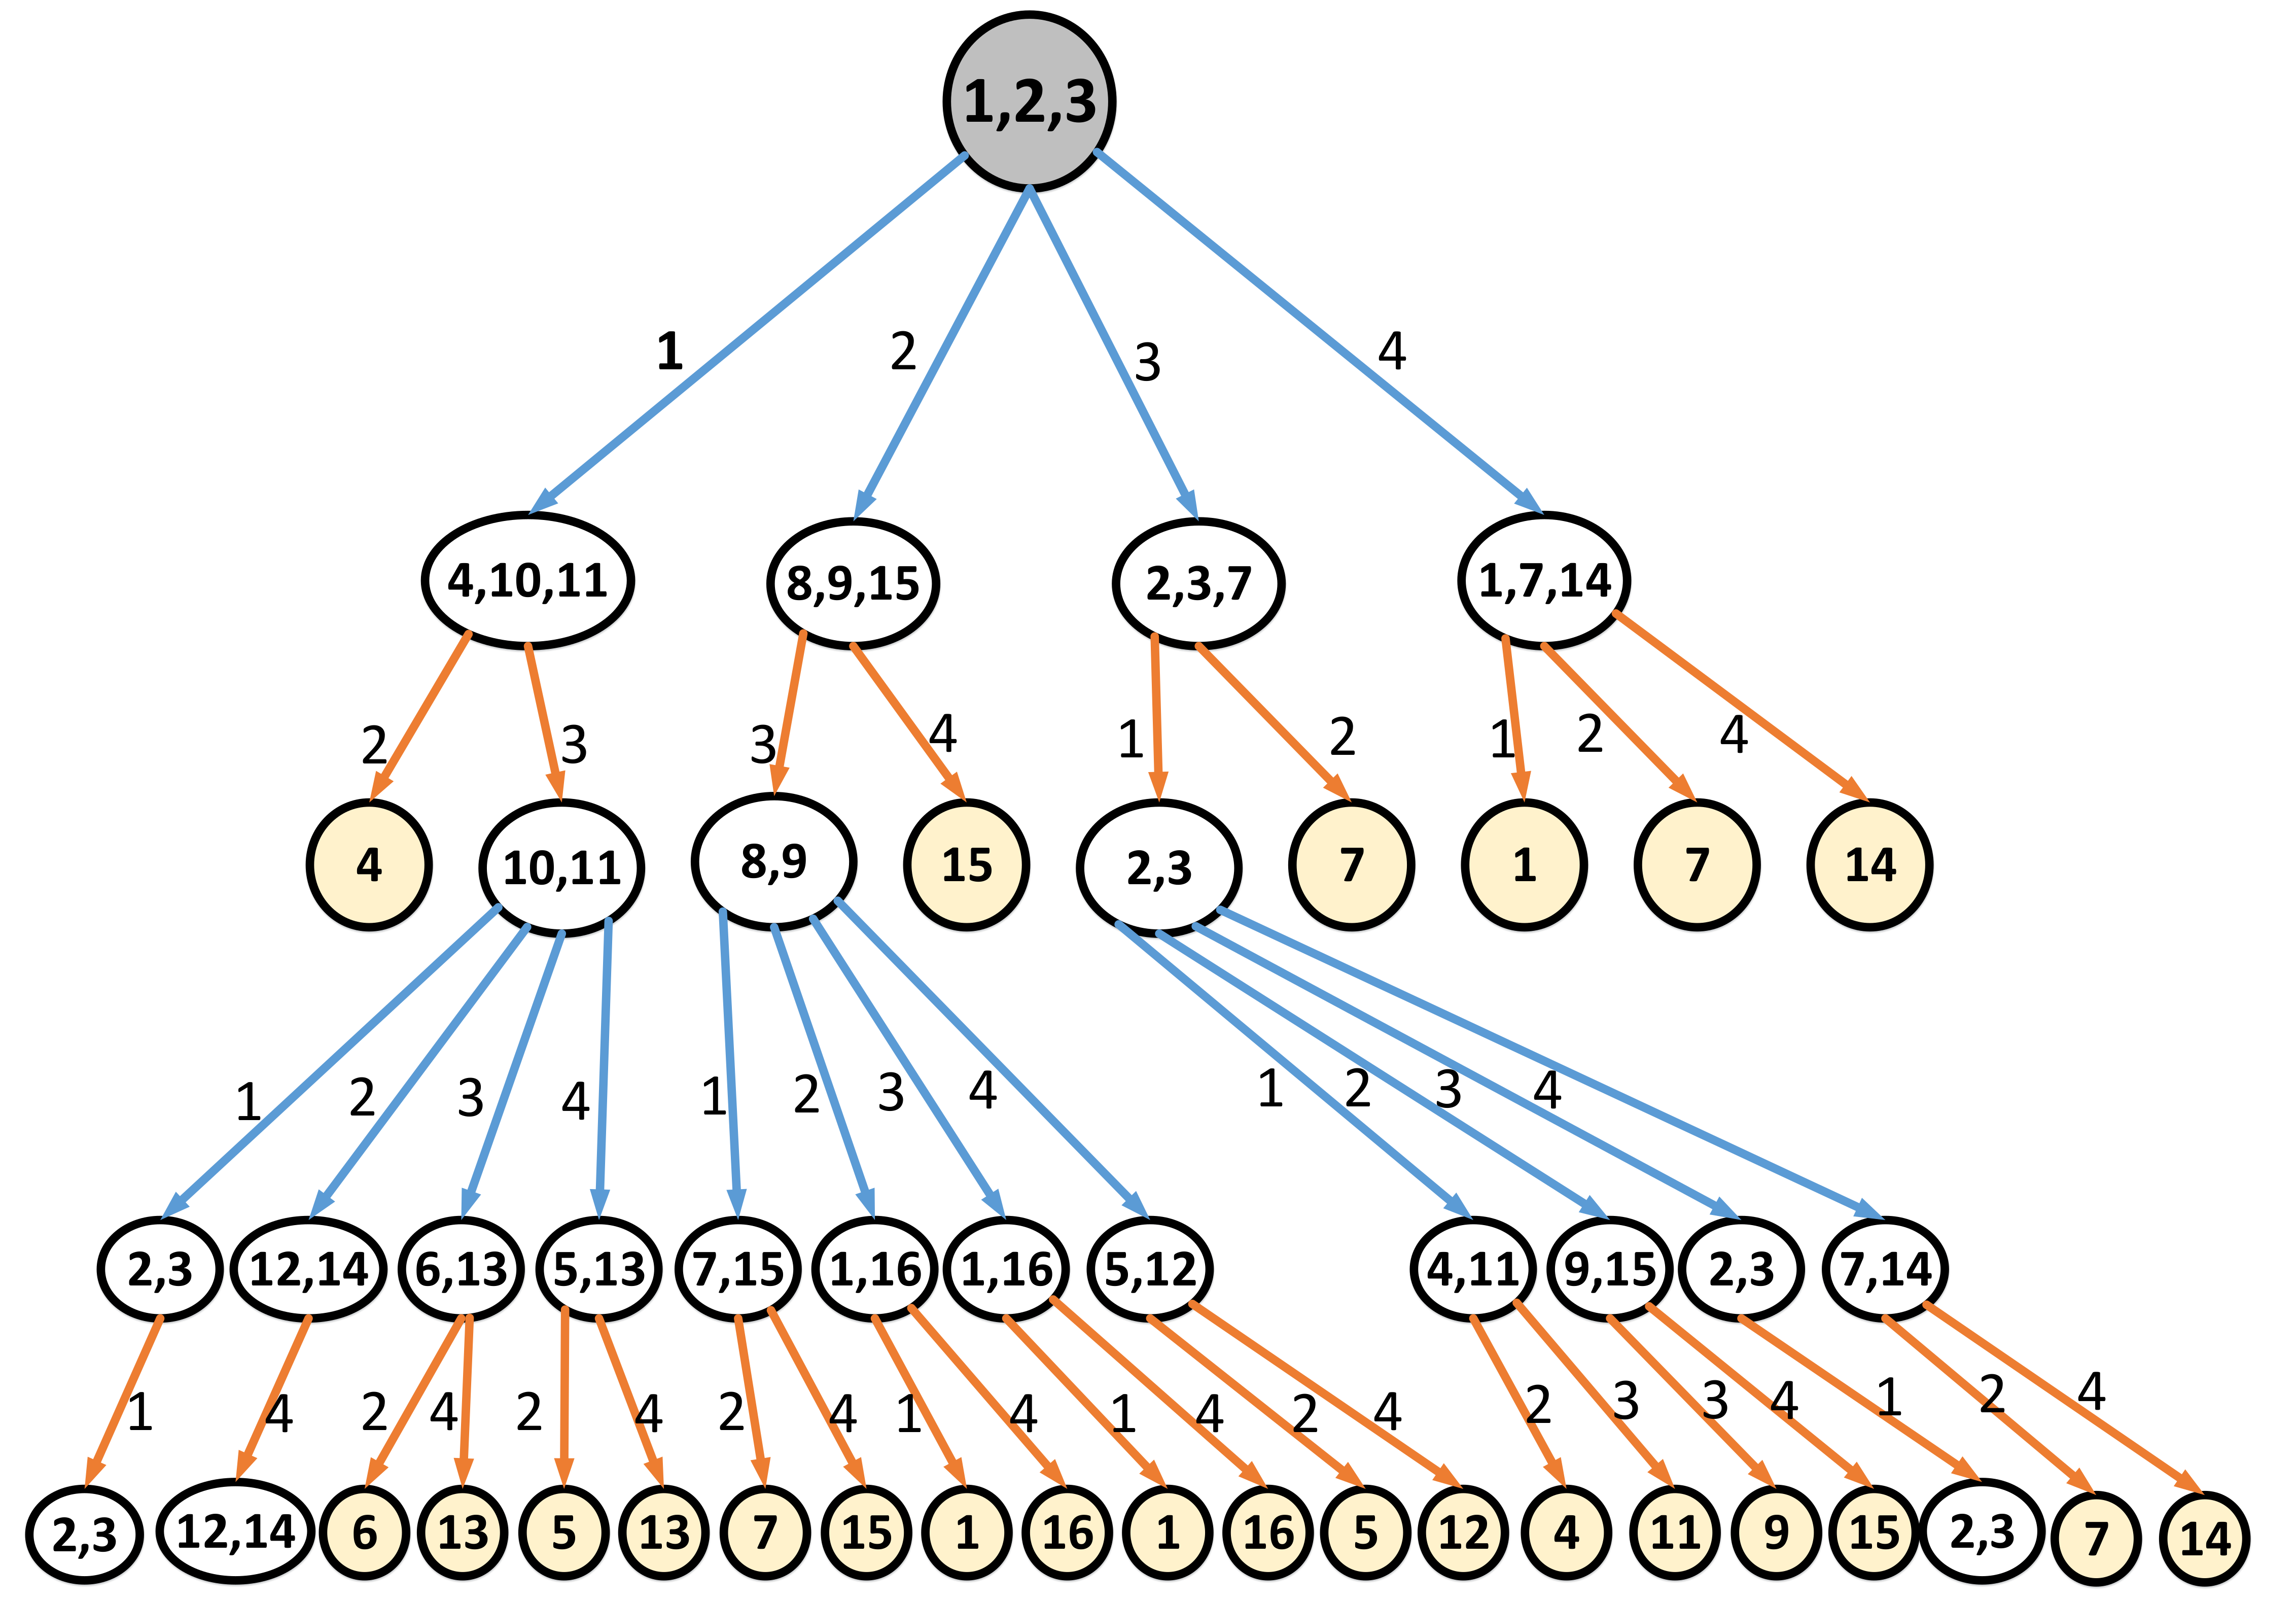
\includegraphics[scale=0.067]{figures/Fig3.png}}
	}}
      
      \caption{Branch of the tree which represents $\{\delta_{16}^1,\delta_{16}^2,\delta_{16}^3\}$. The blue edges and orange edges show the observing output processes and deciding input processes respectively; the yellow nodes are leaf nodes.}
      \label{fig:3}
   \end{figure}

For example, the {\em Fig.\ref{fig:3}} show branch of the tree which represents $\{\delta_{16}^1,\delta_{16}^2,\delta_{16}^3\}$, the nodes represent the states sets, the blue edges represent the observing output processes, and the orange edges represent the deciding input processes. And only the yellow nodes are the leave nodes, so you can see that this branch is not completed. If we want to find all of the ways to determine the initial state, we have to build the complete tree, it will takes many additional time and space overhead. Especially when there are loops in the tree like the $\{\delta_{16}^2,\delta_{16}^3\}$ in fourth layer and the $\{\delta_{16}^2,\delta_{16}^3\}$ in fifth layer that will form a loop. In this case you can never build the complete tree, so you need to check the existence of loops and omit it. There are also some nodes take the same states set which will also take additional overhead, like that there two nodes which take $\{\delta_{16}^1,\delta_{16}^{16}\}$ in the fifth layer. But if we only need to find a ways to determine the initial state, when we find the leaf nodes $\delta_{16}^1$, $\delta_{16}^7$ and  $\delta_{16}^{14}$ in third layer by breadth-first algorithm, you can make sure that the states set $\{\delta_{16}^1,\delta_{16}^2,\delta_{16}^3\}$ is 1 step deterministic.  
\subsection{Directed Graph}
To improve the shortcomings of the way by supertree, we proposed derected graph wich will takes less time and space overhead. The most difference between supertree and derected graph is that supertree is built from the root node to leaf nodes, but the derected graph is built from smaller nodes (contain less states) to larger nodes (contain more states). The construction algorithm of derected graph is showed in the {\em Algorithm 1}, the algorithm to build nodes used in the {\em Algorithm 1} is showed in the {\em Algorithm 2}.

And the way to check whether this input can make the nodes $z$ ($z\ge0$) steps deterministic: According to the order determined in previous steps, we check every node one by one. If for one input $I_i$ which belongs to suitable inputs set of the states set $S_i$ implies $|D\left(S_i,I_i,\varepsilon\right)|<|S_i|$, we can make sure the $I_i$ is a wrong input; else if for all $O_i \in \Delta_Q$ and $|D\left(S_i,I_i,O_i\right)|>0$, the $D\left(S_i,I_i,O_i\right)$ is $Z$ ($Z\ge 0$) steps deterministic then $I_i$ is a right input, then connect the node $S_i$ to all nodes $D\left(S_i,I_i,O_i\right)$ with directed edges, the colour of directed edges represent the corresponding input; else if there exist $O_i \in \Delta_Q$ and we can not make sure whether $D\left(S_i,I_i,O_i\right)$ is $Z$ steps deterministic, we check it in the next round. 
\begin{algorithm}[h]
\caption{Algorithm to construct the directed graph of BCNs}
\begin{algorithmic}[1]
\REQUIRE 
The algebraic forms of BCN
\ENSURE  
The directed graph of BCN
\STATE Define a int variable $k=0$, to represent the number of states in the nodes.\
\STATE Define a boolean type variable $Ob=0$, to represent the online observability of BCN.\
\WHILE {buildnode(k)==1}
\STATE $k= k+1$
\IF{$k==2$}
\STATE We make $\Delta_M$ as the suitable inputs set for every node with $k$ states.
\ELSE
\IF{$k>2$}
\STATE We use two nodes with $(k-1)$ states and a node with two states to find the suitable inputs set for every node with $k$ states. (For example, we can search inputs sets which make $\{\delta_{16}^4,\delta_{16}^5,\delta_{16}^6\}$, $\{\delta_{16}^5,\delta_{16}^6,\delta_{16}^7\}$ and $\{\delta_{16}^4,\delta_{16}^7\}$ $z$ ($z\ge0$) steps deterministic, and then take the intersection of these sets to be the suitable inputs set of $\{\delta_{16}^4,\delta_{16}^5,\delta_{16}^6,\delta_{16}^7\}$.) 
\ENDIF
\ENDIF
\FOR{every node with $k$ states}
\FOR{every input in the suitable input set of the nodes}
\STATE Check whether this input can make the nodes $z$ ($z\ge0$) steps deterministic, and build edges for this node.
\ENDFOR
\ENDFOR
\IF {there exist one node without any edge connect it with other nodes}
\STATE $Ob=0$ return Ob
\ENDIF
\ENDWHILE
\STATE $Ob=1$ return Ob
\end{algorithmic}
\end{algorithm}
\begin{algorithm}[h]
\caption{Algorithm to build nodes with $k$ states}
\begin{algorithmic}[1]
\REQUIRE 
The number of states in the nodes $p$
\ENSURE  
The nodes with $p$ states
\STATE int buildnode(int p)
\STATE  \{ 
\STATE $p=p+1$\
\STATE  Try to build all the nodes with $p$ states whose corresponding outputs are the same, and classify them by their corresponding outputs.\
\IF{Failed to build} 
\STATE  return 0;
\ELSE 
\STATE Sort the states inside the nodes from small to large, and then sort the nodes based on the values inside the nodes. (For example, the nodes $\{\delta_{16}^1,\delta_{16}^2\}$, $\{\delta_{16}^1,\delta_{16}^3\}$ and $\{\delta_{16}^2,\delta_{16}^3\}$ shown in {\em Fig.\ref{fig:4}}. )
\STATE return 1;
\ENDIF 
\STATE \}
\end{algorithmic}
\end{algorithm}
\begin{comment}
\begin{algorithm}
\caption{Calculate $y = x^n$} 
\label{alg1}\begin{algorithmic}
\REQUIRE $n \geq 0 \vee x \neq 0$ 
\ENSURE $y = x^n$ 
\STATE $y \Leftarrow 1$ 
\IF{$n < 0$} 
\STATE $X \Leftarrow 1 / x$ 
\STATE $N \Leftarrow -n$ 
\ELSE 
\STATE $X \Leftarrow x$ 
\STATE $N \Leftarrow n$
\ENDIF 
\WHILE{$N \neq 0$} 
\IF{$N$ is even} 
\STATE $X \Leftarrow X \times X$ 
\STATE $N \Leftarrow N / 2$ 
\ELSE[$N$ is odd] 
\STATE $y \Leftarrow y \times X$ 
\STATE $N \Leftarrow N - 1$ 
\ENDIF 
\ENDWHILE\end{algorithmic}\end{algorithm}


\FOR{each $i \in [1,9]$}
\STATE initialize a tree $T_{i}$ with only a leaf (the root);\
\STATE $T=T \cup T_{i};$\
\ENDFOR
\FORALL {$c$ such that $c \in RecentMBatch(E_{n-1})$} 
\label{code:TrainBase:getc}
\STATE $T=T \cup PosSample(c)$; 
\label{code:TrainBase:pos}
\ENDFOR
\FOR{$i=1$; $i<n$; $i++$ }
\STATE $//$ Your source here;
\ENDFOR
\FOR{$i=1$ to $n$}
\STATE $//$ Your source here;
\ENDFOR
\STATE $//$ Reusing recent base classifiers. 
\label{code:recentStart}
\WHILE {$(|E_n| \leq L_1 )and( D \neq \phi)$}
\STATE Selecting the most recent classifier $c_i$ from $D$;
\STATE $D=D-c_i$;
\STATE $E_n=E_n+c_i$;
\ENDWHILE 
\label{code:recentEnd}
\end{comment}

According the construction process, we have the definition of directed graph.
\begin{definition}[Directed Graph]
For every node $S_i$ in the directed graph, there exists $ K \ge 0$ implies $S_i$ is $K$ stepes deterministic; for every distinct two $s_a, s_b \in S_i$ we have $Hs_a=Hs_b$; if $|S_i|=1$ there are not edge from it to other nodes, else if there are exist one edge contains $I_i$ from it to other nodes then there exist $p$ ($p\ge 1)$ edges contain $I_i$ from it to nodes $S_1,...,S_p$ that $|S_i|= |S_1|+,...,|S_p|$ and $D\left(S_i,I_i,\varepsilon\right)=S_1\vee,...,\vee S_p$.
\end{definition}

We can also use the directed graph to determine the existed second and fourth kinds of observability. When we trying to build bottom layer and penultimate layer of the directed graph, and if there are exist some nodes in penultimate layer has no edges from it to other nodes, then this BCN is not satisfied existed second observability. When we trying to build edges for every layer, and is there exist one node whose right inputs set is not $\Delta_M$, then this BCN is not satisfied existed fourth observability.
\begin{figure}[thpb]
      \centering
      \framebox{\parbox{3in}{
		\centerline{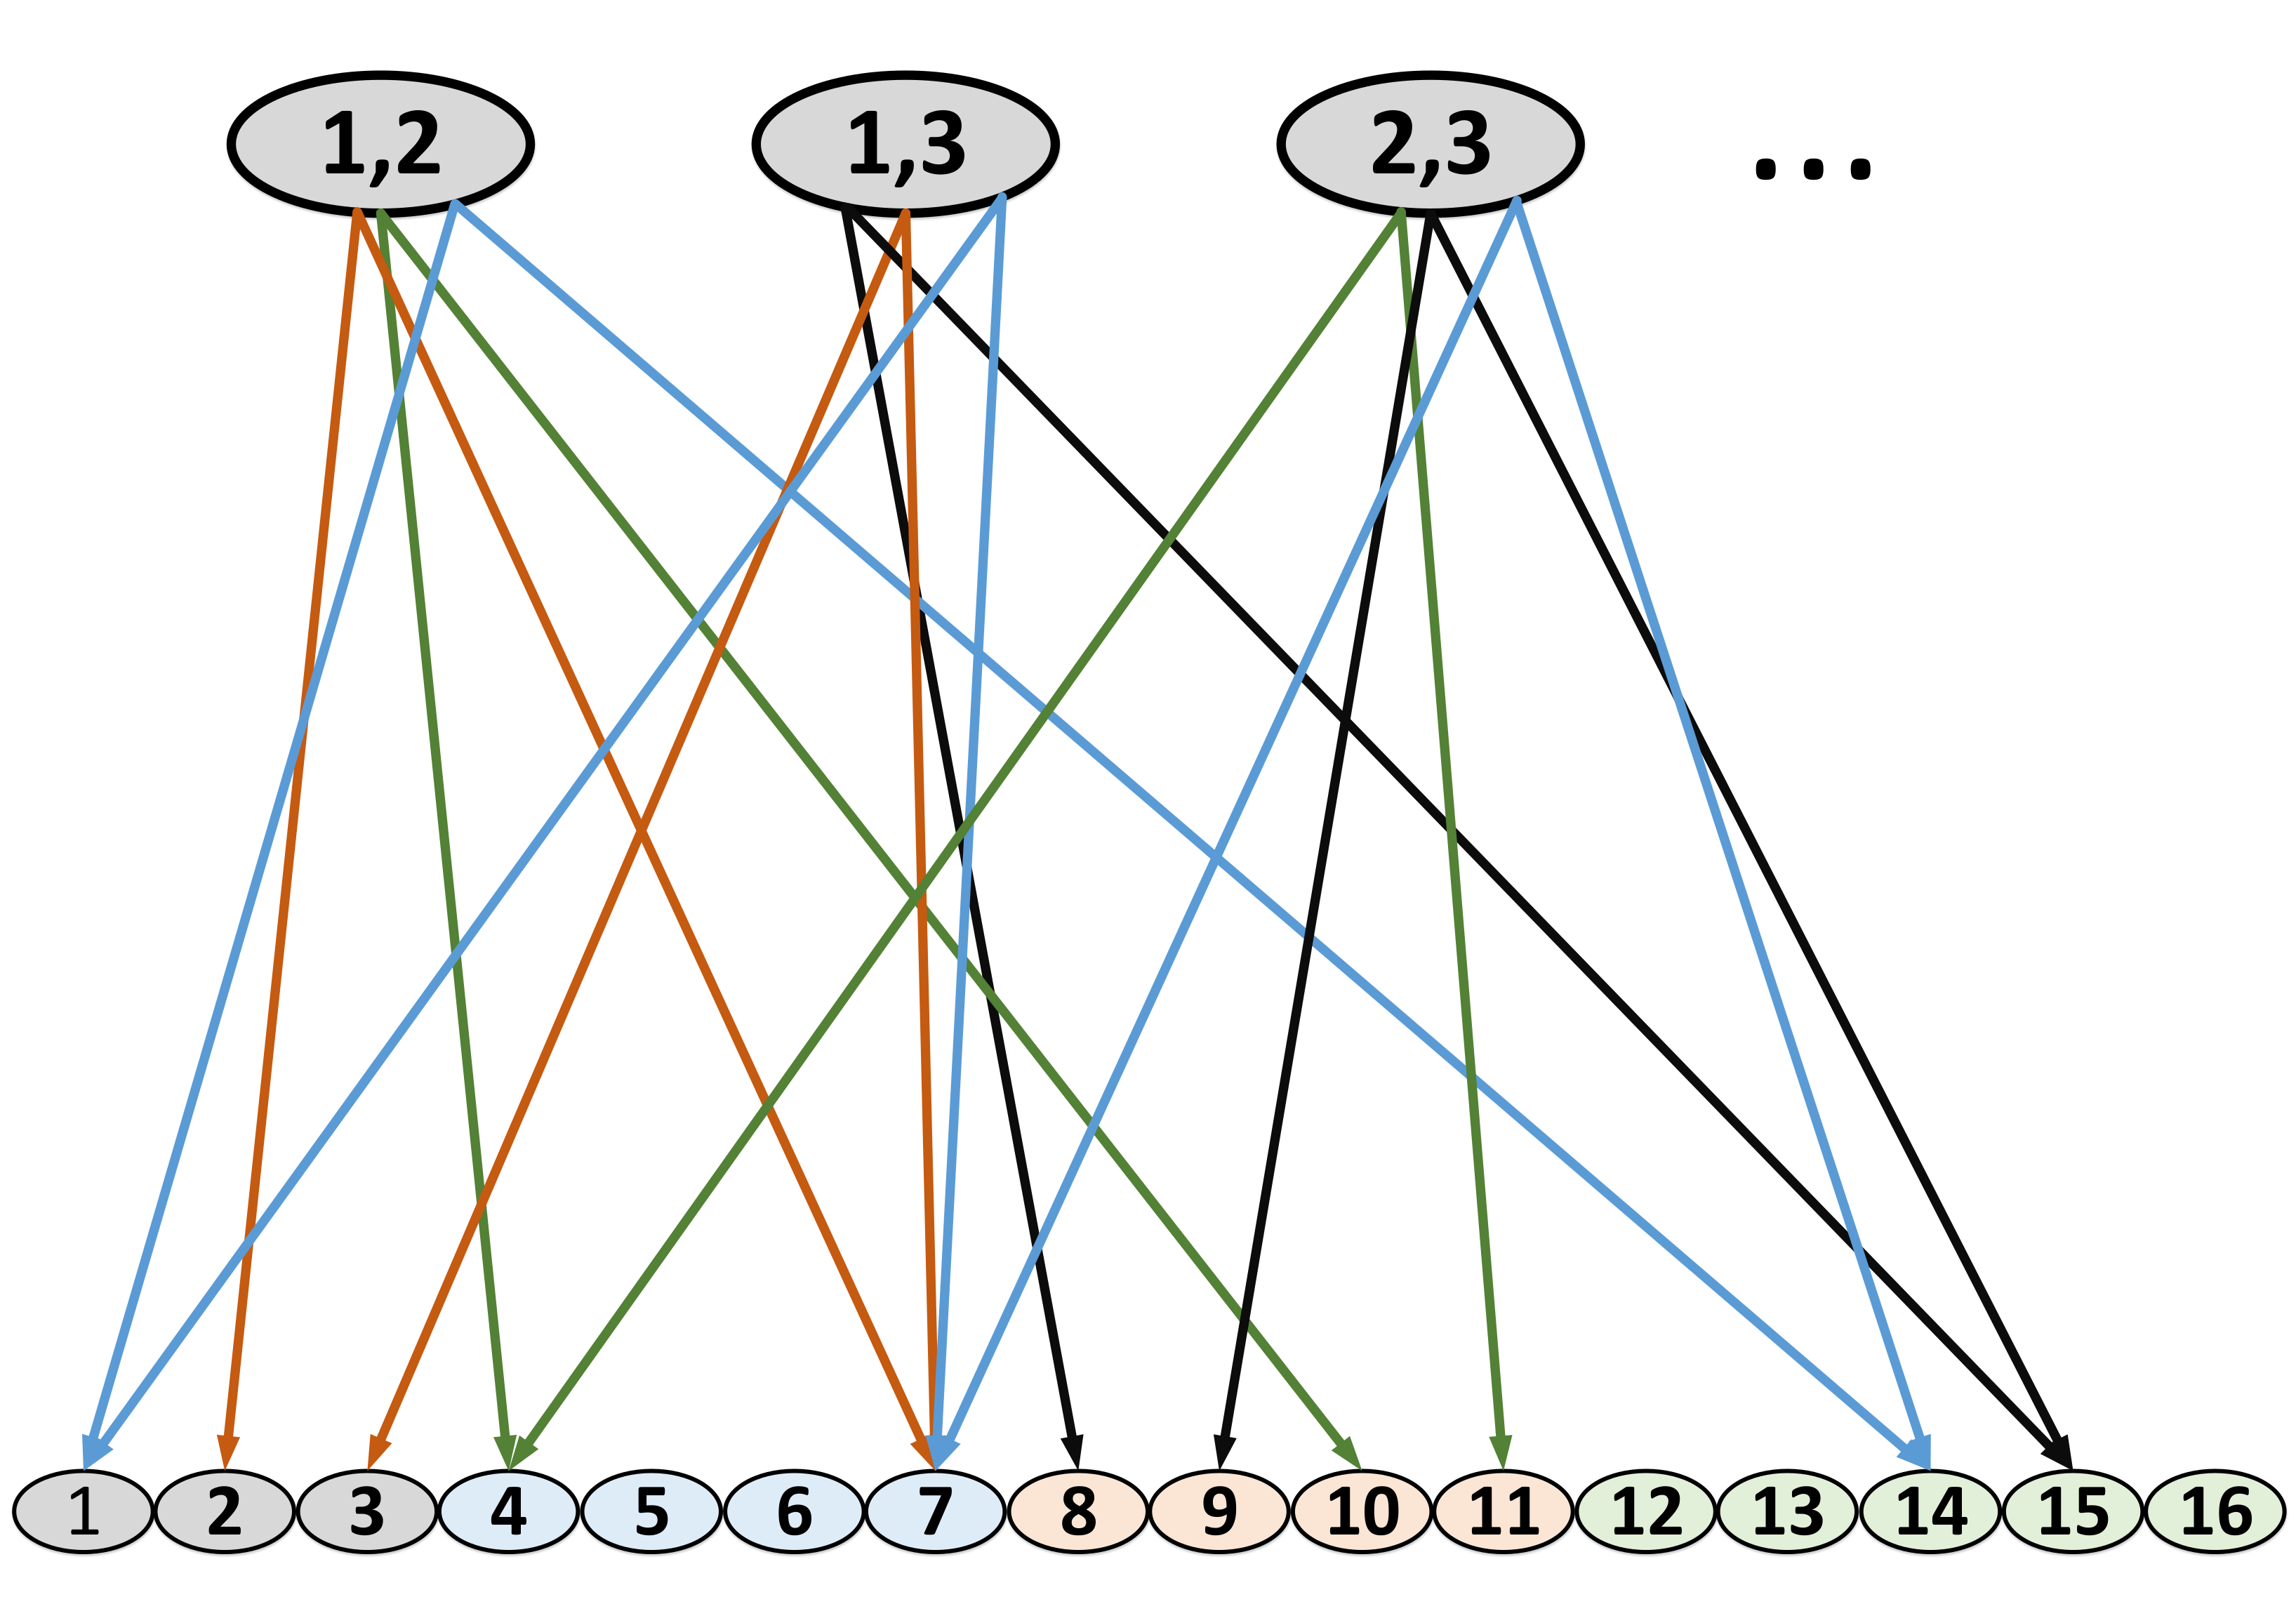
\includegraphics[scale=0.090]{figures/Fig4.png}}
	}}
      
      \caption{Part of the directed graph which represents $\{\delta_{16}^1,\delta_{16}^2\}$, $\{\delta_{16}^1,\delta_{16}^3\}$ and $\{\delta_{16}^2,\delta_{16}^3\}$. The green, black, orange, blue edges show the inputs $\delta_4^1$, $\delta_4^2$, $\delta_4^3$ and $\delta_4^4$ respectively.}
      \label{fig:4}
   \end{figure}
\subsection{Complexity Analysis}
The way use the directed graph to determine the online observability of \BCNs\ is better than by supertree, so we analyze the complexity of it. We classify the states with their corresponding output and form the set of states with the same corresponding output: $S_1$, $S_2$,...,$S_M$.

Firstly, we need to calculate the upper bound of the number of the states in a directed graph nodes $k$, then :
\begin{equation}
\begin{split}
k_{upb}= Max(|S_1|,|S_2|,...,|S_M|)
\end{split}
\end{equation}

Secondly, the number of each nodes with $k$ states:
\begin{equation}
\begin{split}
k_{non}= C_{|S_i|}^k+,...+C_{|S_p|}^k
\end{split}
\end{equation}
where $|S_i|,...,|S_p|\ge k$.

And then the the cardinal number of suitable inputs set of each node, and the time used to check each input is a right input for a node. Finally, calculate the complexity by layer by layer. But the cardinal number of suitable inputs set of a node depends on the number of the states in it, and the other three nodes which used to find the suitable inputs set for it. And the time used to check an input is a right input for  a node of directed graph also depends on the update rules of the {\em BCNs}. So it is hard to give a accurate complexity of the algorithm without the complete imformation of {\em BCNs}.

We can use other three nodes like $\{\delta_{16}^4,\delta_{16}^5,\delta_{16}^6\}$, $\{\delta_{16}^5,\delta_{16}^6,\delta_{16}^7\}$ and $\{\delta_{16}^4,\delta_{16}^7\}$ which is $z$ ($z\ge0$) steps deterministic to find suitable inputs set for $\{\delta_{16}^4,\delta_{16}^5,\delta_{16}^6,\delta_{16}^7\}$. Because only the input which make the subset of $\{\delta_{16}^4,\delta_{16}^5,\delta_{16}^6,\delta_{16}^7\}$ $z$ steps deterministic will make the $\{\delta_{16}^4,\delta_{16}^5,\delta_{16}^6,\delta_{16}^7\}$ $z$ steps deterministic, and use the this three nodes will be a convenient way to cover all the subset of $\{\delta_{16}^4,\delta_{16}^5,\delta_{16}^6,\delta_{16}^7\}$ which with cardinal number 2. By this way we can  reduce the cardinal number of suitable inputs set for every nodes with more than 2 states, then reduce the time cost. 
%Because the states in a nodes will have the same corresponding output, so we have the upper bound of the number of the states in a directed graph nodes $k$: We classify the states with their corresponding output and form the set of states with the same corresponding output, the greatest cardinal number of these set would be the upper bound of $k$. 



\section{APPLICATIONS}

If the \BCN\ we research is online observable, and we have built the directed graph for it, then we can use  it to determine the initial state of {\em BCN}. And we can also use it to try to find the shortest path or avoid entering critical states when we determine the initial state of {\em BCN}. Because the output we observe is undeterminable, we use expected value and variance of the length of path and the times of entering critical states to help us to chose the input.

\subsection{Determine the Initial State}

After we build the directed graph of the {\em BCN}, we can use it to determine the initial state of \BCNs\ as {\em Fig.\ref{fig:5}} shows. First, we observe the output of the {\em BCN} mentioned before, if we observe $\delta_4^1$ that we can infer that the possible states set should be $\{\delta_{16}^1,\delta_{16}^2,\delta_{16}^3\}$, record them as initial states and current states in the table. And then, we input  $\delta_4^1$ and observe  $\delta_4^3$, we can infer that the possible states set can be $\{\delta_{16}^{10},\delta_{16}^{11}\}$, record them as current states set in the corresponding position. Input and output again and again untill we can infer only one  possible state, in that time we can determine the current state and the corresponding initial state of the {\em BCN}.

\begin{figure}[thpb]
      \centering
      \framebox{\parbox{3in}{
		\centerline{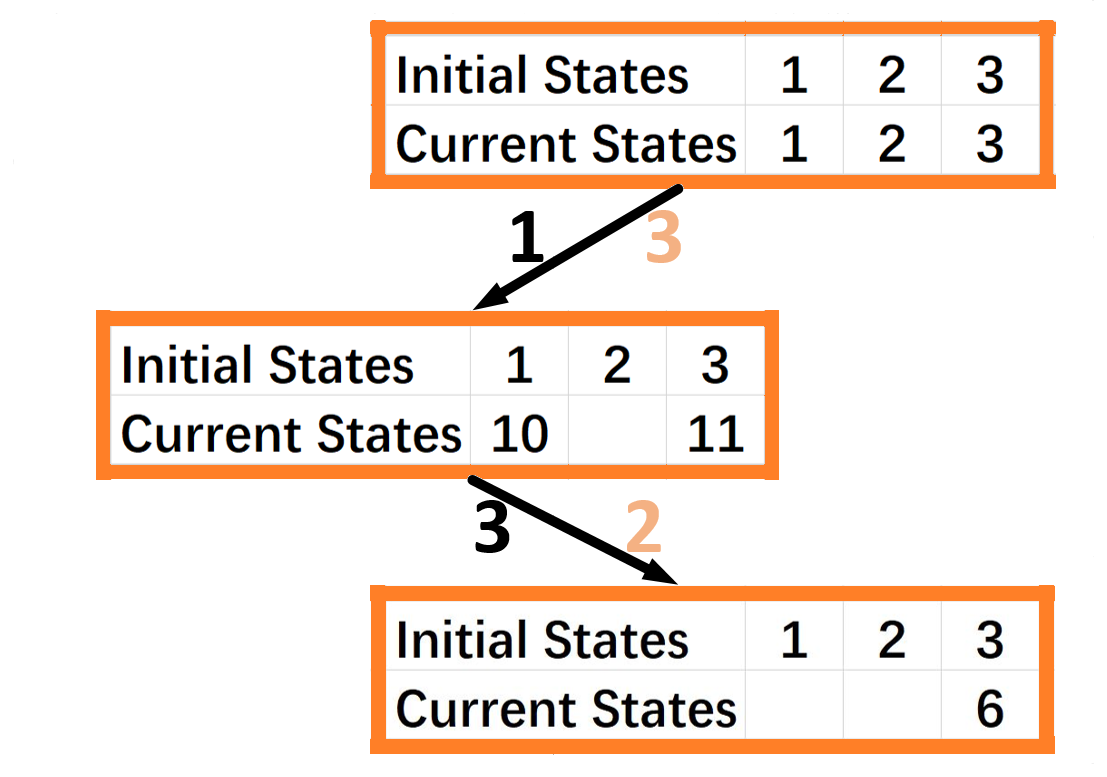
\includegraphics[scale=0.266]{figures/Fig5.png}}
	}}
      
      \caption{The process of determing the initial state of BCNs, we change the values of current states by input and the output we observe. }
      \label{fig:5}
   \end{figure}
\subsection{Less Observation Costs}
Some biological systems, such as the immune systems which can be depicted as the \BCN\ T-cell receptor kinetics model \cite{Klamt2006A}. There exist $3$ input-nodes, and $37$ state-nodes in this model, therefore the model has $2^3$ inputs and $2^{37}$ states. For the purpose of obtain the initial state of the {\em BCN}, one must select some state-nodes to be observe at first. 

And if we use the online observability of \BCNs\ to determine the initial state of the \BCN\ T-cell receptor kinetics model, it will needs less observation costs. Compares with the existed third and fourth kind of observabilities which can also determine the initial state, the online observability need weaker preconditions. Then the online observability needs less output-nodes to be observe and less observation costs. In addition to this, there are also some other advantages, when we use the online observability of {\em BCNs}.

\subsection{Find Shortest Path}
When we need to determine the initial state of a {\em BCN}, an important aspect that we will consider is to find the shortest path. Maybe we can't find the shortest path definitely, but we can use the directed graph to make the best decision. We introduce two functions $Spe(S_i, I_i)$ and $Spv(S_i, I_i)$ to describe the shortest path expected value and shortest path variance, $S_i$ is the possible states set and $I_i$ is the input we chose, the definition of $Spe(S_i, I_i)$ is as follows:\\

\begin{definition}[$Spe(S_i, I_i)$] 
When the $|S_i|=1$, and for every $I_i$ in $\Delta_M$, we have $Spe(S_i, I_i)=0$, then the least shortest path  expected value $Lspe(S_i)= 0$. 
But when the $|S_i|>1$,
 the $\{I_1,I_2,....\}$ is the right inputs set of $S_i$. For every $I_i$ in $\{I_1,I_2,....\}$ the $\{S_i^1,S_i^2,....\}$ is a set of state sets whose elements corresponding to all possible output $O_i$ after input $I_i$, then we have that the $Spe(S_i, I_i)=1 +( (Lspe(S_i^1)|S_i^1|+Lspe(S_i^2)|S_i^2|+....)\left. \right/ |S_i|)$ and $Lspe(S_i)= Min(Spe(S_i, I_1),Spe(S_i, I_2),...)$.
\end{definition}
\subsection{Avoid Entering Critical States}
In biological systems, some states of the genes may corresponding to unfavorable or dangerous situations \cite{Li2014Controllability}. So another important aspect that we will consider is to avoid entering critical states. We can also construct two functions $Lce(S_i, I_i)$ and $Lcv(S_i, I_i)$ to describe least expected value and variance of the times of entering critical states, the definition of $Lce(S_i, I_i)$ is as follows:\\

\begin{definition}[$Lce(S_i, I_i)$] 
When the $|S_i|=1$, and for every $I_i \in \Delta_M$, we have $Lce(S_i, I_i)=|S_i \cap CS |$, then the least shortest path  expected value $Llce(S_i)=|S_i \cap CS |$. 
But when the $|S_i|>1$, 
the $\{I_1,I_2,....\}$ is the right inputs set of $S_i$. For every $ I_i$ in $\{I_1,I_2,....\}$ the $\{S_i^1,S_i^2,....\}$ is a set of state sets whose elements corresponding to all possible output $O_i$ after input $I_i$, then we have $Lce(S_i, I_i)=(|S_i \cap CS | + (Llce(S_i^1)|S_i^1|+Llce(S_i^2)|S_i^2|+....)\left. \right/ |S_i|)$ and $Llce(S_i)= Min(Lce(S_i, I_1),Lce(S_i, I_2),...)$.
\end{definition}

Where the $CS$ is the critical states set of the {\em BCN} we research.\\

Then we can get the definitions of $Spv(S_i, I_i)$ and $Lcv(S_i, I_i)$ in similar ways, and use them to make the best decision we like. When we choos an input with least $Spe(S_i, I_i)$, we may find the shortes path to determine the initial state. But the output of \BCNs\ is uncertain, so selected the least $Spe(S_i, I_i)$ may leads to a very long path. For better performce, we the can also use the $Spv(S_i, I_i)$ to avoiding risks. The uses of $Lce(S_i, I_i)$ and $Lcv(S_i, I_i)$ are similar to $Spe(S_i, I_i)$ and $Spv(S_i, I_i)$, when we trying to avoid entering critical states of {\em BCNs}.

In the existed four kinds of observability, we can not analyze the state of \BCNs\ dynamically, maybe it would be a little hard to find the best way we like to determine the initial state of {\em BCNs}.
\section{CONCLUSIONS}

In this paper, we proposed online observability of {\em BCNs} and define its mathematical form;  then we use the super tree and directed graph to determine the online observability; after determined the online observability we use it to try to find the shortest path and avoid entering critical states when we determining the initial state of {\em BCNs}. 

But even we use the directed graph, it is still hard to determine the  the online observability of \BCNs\ which with a large number of nodes. So, in the future we will try to separate the {\em BCNs}, and then determine their online observability; and try to use some knowledge about formal methods for better scalable of {\em BCNs}. In addition to the theoretical aspects, the realistic application is also very important, we will also try to find some realistic example which can be modeled by {\em BCNs}, then determine their online observability for better performance.
\addtolength{\textheight}{-12cm}   % This command serves to balance the column lengths
                                  % on the last page of the document manually. It shortens
                                  % the textheight of the last page by a suitable amount.
                                  % This command does not take effect until the next page
                                  % so it should come on the page before the last. Make
                                  % sure that you do not shorten the textheight too much.

%%%%%%%%%%%%%%%%%%%%%%%%%%%%%%%%%%%%%%%%%%%%%%%%%%%%%%%%%%%%%%%%%%%%%%%%%%%%%%%%



%%%%%%%%%%%%%%%%%%%%%%%%%%%%%%%%%%%%%%%%%%%%%%%%%%%%%%%%%%%%%%%%%%%%%%%%%%%%%%%%



%%%%%%%%%%%%%%%%%%%%%%%%%%%%%%%%%%%%%%%%%%%%%%%%%%%%%%%%%%%%%%%%%%%%%%%%%%%%%%%%
\begin{comment}
\section*{APPENDIX}

Appendixes should appear before the acknowledgment.

\section*{ACKNOWLEDGMENT}

The preferred spelling of the word �acknowledgment� in America is without an �e� after the �g�. Avoid the stilted expression, �One of us (R. B. G.) thanks . . .�  Instead, try �R. B. G. thanks�. Put sponsor acknowledgments in the unnumbered footnote on the first page.
\end{comment}


%%%%%%%%%%%%%%%%%%%%%%%%%%%%%%%%%%%%%%%%%%%%%%%%%%%%%%%%%%%%%%%%%%%%%%%%%%%%%%%%

%References are important to the reader; therefore, each citation must be complete and correct. If at all possible, references should be commonly available publications.

 \bibliographystyle{IEEEtran} 

 \bibliography{bcn}
 


\end{document}
